\section{Deep Neural Networks}
In this section, we give a brief review of the deep learning architectures that we used
in network intrusion detection problem.

\subsection{Multilayer Perceptron}
Multilayer perceptron (MLP) is the simplest deep learning classifier in terms of
design of the architecture.
It is a fully connected feed-forward neural network, as shown in Figure~\ref{Fig:MLPArchitecture}.
By introducing non-linear neural units (perceptron), it can distinguish data that are
not linearly separable.
However, the non-linearity also make it very hard to train a deep MLP,
even if people have proposed the efficient back-propagation learning algorithm~\cite{Backpropagation}.
Recently it revived due to various new training techniques designed by deep learning community,
including Stochastic Gradient Descent (SGD),
batch normalization~\cite{BatchNorm} and Dropout~\cite{Dropout}.
Expect for the number of neurons in each layer and number of layers,
MPL can also be tuned with different activation functions, or neural types.
The most popular two, which are used in this project, are logistic function
and rectifier linear unit.
Logistic function is written as
\begin{align}
        f(x) &= \frac{1}{1 + e^{-x}}
\end{align}
It has a very useful property when we applying backpropagation:
\begin{align}
        f'(x) &= f(x) (1-f(x))
\end{align}
Recently, most deep neural networks adopt rectifier neural unit and achieved very good performance~\cite{DeepLearning}.
Rectifier linear unit is defined as
\begin{align}
        f(x) &= \max(0, x)
\end{align}
Let $\mathbf{a}^{(l)}$ be the activation of layer $l$,
$\mathbf{W}^{(l)}$ and $\mathbf{b}^{(l)}$ be layer $l$'s parameter.
With activation function defined, we have the following recursive formula that describes
the feed-forward step of the perceptron network.
\begin{align}
        \mathbf{z}^{(l+1)} &= \mathbf{W}^{(l)} \mathbf{a}^{(l)} + \mathbf{b}^{(l)} \\
        \mathbf{a}^{(l+1)} &= f(\mathbf{z}^{(l+1)})
\end{align}

\begin{figure}[h]
\centering
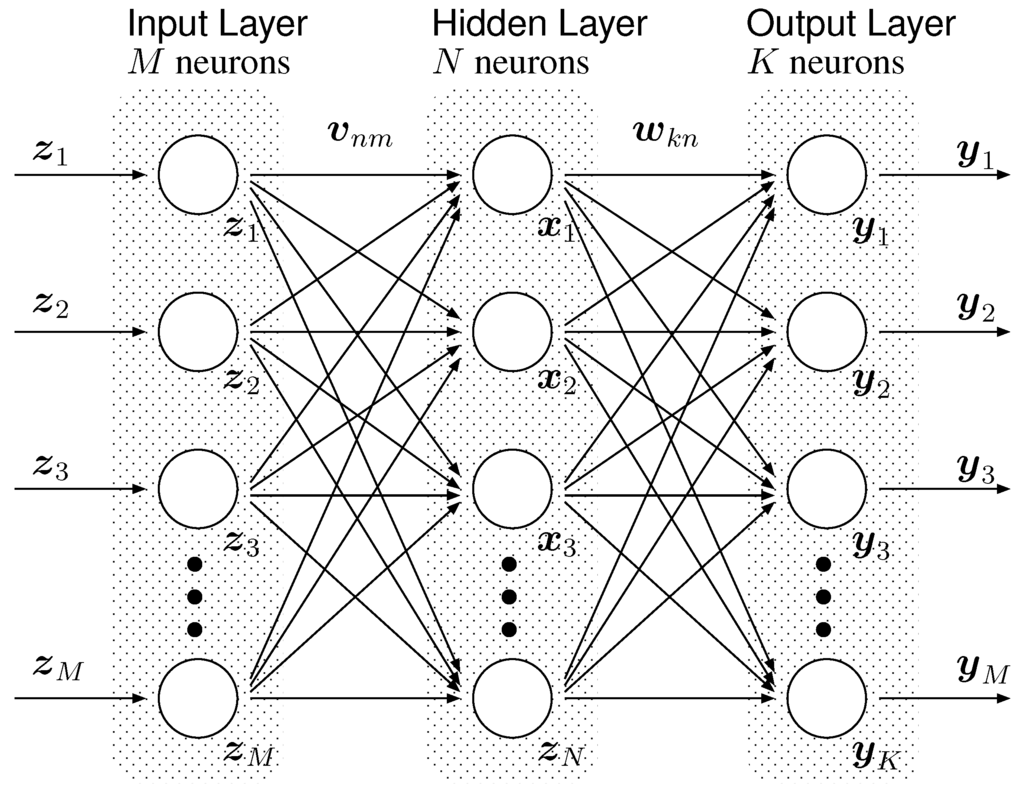
\includegraphics[width=0.45\textwidth]{figures/multilayer_perceptron.png}
\caption{A perceptron neural network with 1 hidden layer.
        Figure courtesy of Teijiro Isokawa, Haruhiko Nishimura and Nobuyuki Matsui.}
\label{Fig:MLPArchitecture}
\end{figure}

\subsection{Generative Models}
The amount of network traffic data is enormously large, usually in the order of terabytes
per day in a large monitored network.
This available big data makes deep learning techniques a promisingly better solution
to traffic classification.
In practice, however, the amount of data is impossible for a human security analyst to review,
e.g., to find patterns and label anomalies.
Generative model which can be trained unsupervisedly comes to rescue in that
\begin{itemize}
\item It utilizes the large amount of unlabeled data to learning useful and hierarchical features;
\item It is actually a way to initialize the weights in a deep neural network, which can be
        further fine-tuned to be a high performance classifier.
\end{itemize}
In this project we propose to try two generative models: restricted Boltzmann machine and autoencoders.

\subsubsection{Restricted Boltzmann Machine}
Restricted Boltzmann machine (RBM) consists of a layer of hidden units (H) and a layer of visible units (V).
Here, ``restricted" means that connections are just between hidden and visible layer,
but not within hidden layers or visible layers.
This make training RBM faster than Boltzmann machine and feasible for stacking together
to form deep architecture.
After learning the first layer RBM, the activity vector of the hidden units can be used
as ``data" for training the second layer RBM
and this process can be repeated to learn as many hidden layers as desired.
As data passing through the RBMs, we can obtain the highest level features 
which are typically fed into a classifier.
The entire deep network (RBMs plus the classifier) can be fine-tuned to
improve the classification performance.

\begin{align}
        E(\mathbf{v, h}) &= -\sum_i b_i v_i - \sum_j b_j h_j - \sum_{i, j} v_i h_j w_{ij} \\
        \Delta w_{ij} &= \epsilon (<v_i h_j>_{data} - <v_i h_j>_{reconstruction}) \\
        Prob(h_j = 1) &= sigmoid(b_j + \sum_i{v_i w_{ij}}) \\
\end{align}



\subsubsection{Autoencoders}
An autoencoder neural network is an unsupervised model with typically one hidden layer that
tries to set the output layer to be equal to the input.
As shown in Figure~\ref{Fig:AEArchitecture}, we want the network to
learn a function $h_{W, b}(x) \approx x$.
However, to prevent the network from learning the meaningless identify function,
we need to place extra constraints on the network, which introduces many different
flavors of autoencoders.
In this project we consider two most popular type of autoencoders, sparse autoencoder and
denoise autoencoder.

The \textbf{denoising autoencoder} algorithm is proposed by~\cite{DenoiseAE} and illustrated in
Figure~\ref{Fig:dAEAlgorithm}.
To prevent learning identify function, an example $\mathbf{x}$ is first corrupted, either by
adding Gaussian noise or by random masking a fraction of items in $\mathbf{x}$ to zero.
The autoencoder then maps corrupted $\mathbf{\tilde{x}}$ to a hidden representation $\mathbf{y} = sigmoid(\mathbf{W}\tilde{\mathbf{x}} + \mathbf{b})$.
From $\mathbf{y}$ we reconstruct a $\mathbf{z}=g_\theta'(\mathbf{y})$.
The training needs to learning the parameters $\theta$ and $\theta'$ so that average reconstruction error is minimized over training set.
For binary input $\mathbf{x}$, usually cross entropy is adopted as $L_H(\mathbf{x}, \mathbf{z})$;
while mean squared error is used for real-valued $\mathbf{x}$.

\begin{figure}[h]
\centering
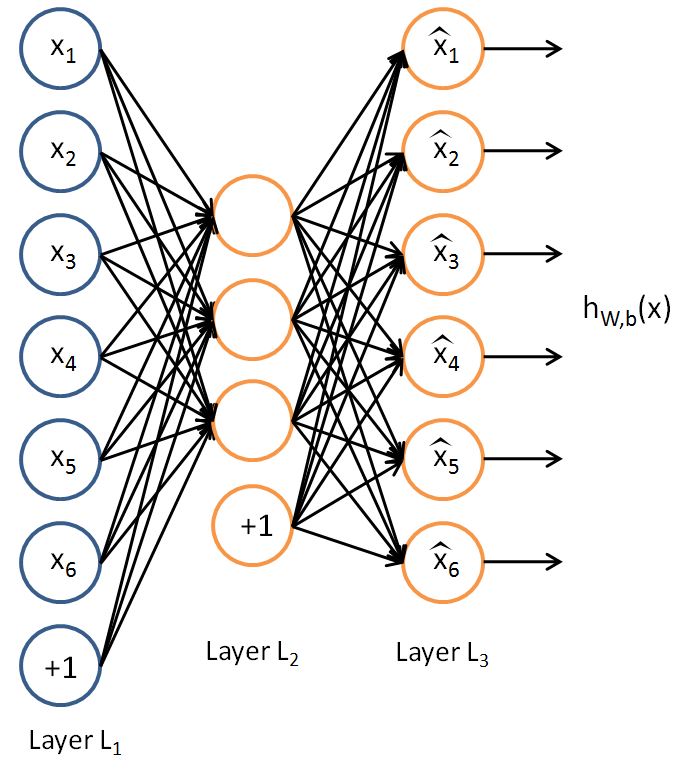
\includegraphics[width=0.45\textwidth]{figures/autoencoder.png}
\caption{General Architecture of Autoencoders.
        Figure courtesy of~\cite{UFLDLAutoencoder}.}
\label{Fig:AEArchitecture}
\end{figure}

\begin{figure}[h]
\centering
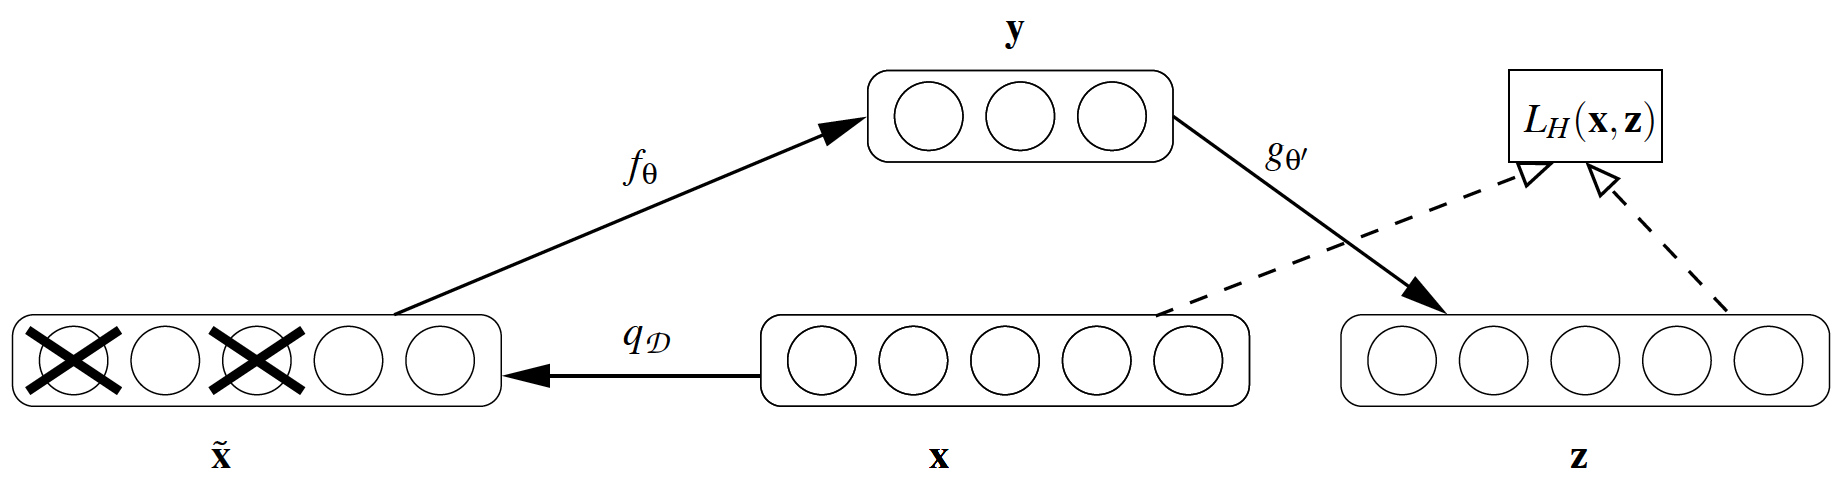
\includegraphics[width=0.45\textwidth]{figures/denoiseautoencoder.png}
        \caption{The denoising autoencoder algorithm.
        Input example $\mathbf{x}$ is randomly corrupted via $q_\mathcal{D}$ and then
        is mapped via encoder $f_\theta$ to $\mathbf{y}$.
        The decoder $g_\theta'$ attempts to reconstruct $\mathbf{x}$ and produces $\mathbf{z}$.
        Reconstruction error is measured by loss $L_H(\mathbf{x}, \mathbf{z})$, to be minimized
        during the training phase.}
\label{Fig:dAEAlgorithm}
\end{figure}

The \textbf{sparse autoencoder} works by placing a sparsity constraint on the hidden units~\cite{SparseAE}.
First, we make the autoencoder's hidden layer size to be over-complete,
that is of larger size comparing to the dimension of the input.
Let's denote the activation of hidden unit $j$ of layer 2 in Figure~\ref{Fig:AEArchitecture}
to be $a^2_j(\mathbf{x})$ given input example $\mathbf{x}$.
With that, we can define the average activation of hidden unit $j$ over the $m$-size
training set
\begin{align}
        \hat{\rho}_j = \frac{1}{m} \sum_{i=1}^{m} a^2_j(\mathbf{x})
\end{align}
The sparsity constraint is enforcing, $\forall$ hidden unit $j$,
\begin{align}
        \hat{\rho}_j = \rho
\end{align}
where $\rho$ is a sparsity parameter that approximates zero (say 0.05).
This constraint can be vectorized over the hidden layer, say of size $n_2$,
with the KL divergence based penalty term
\begin{align}
        \sum_j^{n_2} KL(\rho || \hat{\rho}_j)
        = \sum_j^{n_2} [\rho \log \frac{\rho}{\hat{\rho}_j} + (1 - \rho) \log \frac{1-\rho}{1-\hat{\rho}_j} ]
\end{align}
The sparsity penalty term is integrated into the cost function by adding another hyperparameter $\beta$
\begin{align}
        L(W, b) = \frac{1}{2}||h_{W,b}(\mathbf{x}) - \mathbf{x}||^2 + \beta \sum_j^{n_2} KL(\rho || \hat{\rho}_j)
\end{align}

Denoise autoencoder and sparse autoencoder, surprisingly, have different application domains.
Vincent et al.~\cite{DenoiseAE} have shown that stacked denoise autoencoder can be used to
initialize a deep neural network's weight parameter,
achieving similar and sometimes better performance than stacked RBM.
They also show that training stacked denoise autoencoder with MNIST dataset, it is able
to resynthesize a variety of similarly good quality digits.
Raina et al.~\cite{SparseAE} have compared sparse encoding with principle component analysis
(PCA) and argue that transfer raw features with a well unsupervisely trained
sparse audoencoder can be beneficial to supervised learning algorithm,
for example support vector machine (SVM).
